%=========================================================
\chapter{Pruebas}

El aseguramiento de la calidad es un pilar fundamental en el desarrollo de cualquier sistema de software. En el presente capítulo, se detalla el proceso de validación del sistema propuesto a través de la ejecución de pruebas enfocadas en sus principales casos de uso. El objetivo es verificar que cada funcionalidad crucial del sistema se comporta de acuerdo con las especificaciones y requisitos definidos. 

\section{Pruebas de humo y detección temprana de errores}

Durante la fase de codificación y desarrollo del sistema, se llevó a cabo varias pruebas de humo de manera continua. Estas pruebas informales, realizadas al finalizar cada sección o módulo de código, fueron cruciales para detectar defectos críticos en las etapas más tempranas del ciclo de desarrollo. Esta práctica permitió identificar y corregir errores conforme se presentaban, asegurando la funcionalidad básica de cada componente antes de la integración completa.

Entre los errores más destacables que se identificaron y subsanaron durante estas pruebas iniciales, se encuentran:

\begin{itemize}
	\item \textbf{Errores de formato en la comunicación con el servidor:} Se observó que, en cualquier interacción con el servidor (tanto el de Spring Boot como el de la Red Neuronal), se producían errores de servidor (`Server Error`) si el formato de la información enviada al servidor no coincidía con el esperado o, a la inversa, si la respuesta del servidor no se ajustaba a la estructura de datos que la aplicación móvil estaba preparada para recibir. Esto obligó a una revisión exhaustiva de la serialización y deserialización de datos para garantizar la coherencia.
	
	\item \textbf{Limitación de tamaño de imagen en el módulo de Reconocimiento Facial:} Se identificó un error crítico en el módulo de reconocimiento facial cuando un dispositivo móvil intentaba enviar una fotografía de muy alta resolución o de gran tamaño. El servidor de Azure, donde reside el modelo de red neuronal, cancelaba la petición al exceder los límites de tamaño permitidos, lo que resultaba en fallos de comunicación. La solución implicó la implementación de un proceso de compresión de imágenes en el lado del cliente (la aplicación móvil) antes de su envío.
	
	\item \textbf{Manejo de errores en detección de rostros del módulo de reconocimiento facial:} Otro error significativo en el módulo de reconocimiento facial era que si la imagen enviada al servidor de la red neuronal no contenía un rostro detectable, el servidor fallaba inesperadamente en lugar de retornar un error manejable. Esto causaba un comportamiento no deseado en la aplicación y se requirió una modificación para que el servidor, al no detectar un rostro, respondiera con un error específico que pudiera ser capturado y gestionado adecuadamente por la aplicación móvil, informando al usuario de la situación de manera clara.
\end{itemize}

La detección temprana y corrección de estos y otros errores mediante las pruebas de humo fue vital para el correcto funcionamiento del sistema final, permitiendo avanzar a fases de prueba más formales con una base más sólida.

\section{Pruebas de integración}

Además de las pruebas de humo realizadas durante el desarrollo, se llevaron a cabo pruebas de integración para asegurar que los distintos componentes del sistema interactuaran correctamente entre sí. Estas pruebas se centraron específicamente en la conexión y el flujo de datos entre la aplicación móvil, el servidor de Spring Boot, el servidor de la red neuronal y la simulación del SAES.

El objetivo principal de estas pruebas fue verificar que:
\begin{itemize}
	\item La aplicación móvil pudiera establecer conexiones exitosas con ambos servidores.
	\item Los datos se enviaran y recibieran correctamente entre la aplicación móvil y el servidor de Spring Boot (ej. inicio de sesión, gestión de datos de alumnos/ETS).
	\item La comunicación para el reconocimiento facial funcionara fluidamente entre la aplicación móvil y el servidor de la red neuronal, incluyendo el envío de imágenes y la recepción de resultados de verificación.
	\item La \textbf{simulación del SAES} se conectara adecuadamente con el servidor de la red neuronal para llevar a cabo los procesos de registro de usuarios y la generación de embeddings faciales.
\end{itemize}
Estas pruebas de integración fueron fundamentales para validar la arquitectura de comunicación de los servicios desplegados.

\section{Pruebas de subsistema}

Adicionalmente a las pruebas de humo e integración, se realizaron pruebas de subsistema exhaustivas para verificar el correcto funcionamiento y la interacción de conjuntos específicos de componentes que conforman funcionalidades clave del sistema. Estas pruebas se diseñaron para asegurar que cada módulo principal operara de manera coherente y eficiente, tanto de forma independiente como en conjunto con sus dependencias directas. Los subsistemas clave evaluados incluyen:

\begin{itemize}
	\item \textbf{Gestión y visualización de reportes por docentes:} Se comprobó la funcionalidad completa de la creación y visualización de reportes por parte del personal docente. Esto incluyó la verificación de la generación de reportes de asistencia (con o sin el uso de reconocimiento facial), la correcta agregación de datos y la presentación adecuada de la información en la interfaz de usuario del docente.
	
	\item \textbf{Registro de asistencia escolar por personal de seguridad:} Se validó el flujo completo de registro de asistencia de alumnos a la escuela a través del personal de seguridad. Esta prueba abarcó desde la captura de la identificación del alumno hasta el registro exitoso de su entrada en la base de datos, asegurando la fiabilidad del proceso en los puntos de acceso.
	
	\item \textbf{Verificación de reconocimiento facial por alumnos:} Se realizaron pruebas detalladas sobre la funcionalidad de reconocimiento facial utilizada por los alumnos para verificar su identidad. Esto implicó la verificación de la captura de la imagen, el envío al servidor de la red neuronal y la correcta interpretación de la respuesta para determinar la identidad del alumno.
	
	\item \textbf{Funcionamiento del servidor Spring Boot:} Se sometió el servidor de Spring Boot a pruebas de subsistema intensivas para asegurar el correcto procesamiento de la lógica de negocio, la gestión de la base de datos (PostgreSQL) y la orquestación de las peticiones recibidas desde la aplicación móvil. Esto incluyó la verificación de la autenticación de usuarios, la gestión de datos de alumnos y ETS, y la integridad de las transacciones.
	
	\item \textbf{Funcionamiento de las funciones de creación de Embeddings y reconocimiento facial en el Servidor de la Red Neuronal:} El servidor de la red neuronal fue específicamente probado para validar la exactitud y eficiencia de sus funciones principales. Se verificó el correcto funcionamiento de:
	\begin{itemize}
		\item La \textbf{creación de embeddings}: La capacidad de transformar una imagen facial en un vector numérico único que representa las características faciales.
		\item El \textbf{reconocimiento facial}: La comparación de embeddings para determinar la similitud entre rostros y, por ende, la identidad o no identidad de un individuo.
	\end{itemize}
	Estas pruebas fueron cruciales para asegurar la precisión y el rendimiento del componente de inteligencia artificial.
\end{itemize}

Las pruebas de subsistema permitieron identificar y resolver interacciones complejas entre módulos, garantizando que cada pieza fundamental del sistema funcionara de manera óptima y contribuyera a la robustez general de la solución.

\section{Pruebas de aceptación (encuestas de usuario)}

La fase final de validación del sistema se llevó a cabo mediante pruebas de aceptación de usuario, específicamente a través de la aplicación de encuestas. Estas encuestas fueron diseñadas para recopilar la percepción directa de los usuarios finales (docentes, personal de seguridad y alumnos) sobre la usabilidad, la eficiencia, la satisfacción general y la efectividad del sistema en un entorno cercano al real.

El objetivo principal de estas encuestas fue:
\begin{itemize}
	\item \textbf{Validar la satisfacción del usuario:} Medir el grado en que el sistema cumple con las expectativas y necesidades de los usuarios, más allá de la mera funcionalidad técnica.
	\item \textbf{Identificar oportunidades de mejora:} Recopilar retroalimentación cualitativa y cuantitativa que permita identificar áreas de mejora en la interfaz de usuario, la experiencia de usuario y las funcionalidades futuras del sistema.
	\item \textbf{Confirmar la aceptación del sistema:} Determinar si el sistema es adecuado para su implementación y uso en el entorno operativo previsto, asegurando que los usuarios se sientan cómodos y productivos con la herramienta.
	\item \textbf{Evaluar la efectividad percibida:} Cuantificar la percepción de los usuarios sobre cómo el sistema resuelve los problemas planteados, como la agilización del registro o la prevención de la suplantación de identidad.
\end{itemize}

Los resultados de estas encuestas, analizados detalladamente en el Capítulo de Resultados, fueron cruciales para obtener una perspectiva valiosa sobre la experiencia de usuario y confirmaron la viabilidad y aceptación del sistema en el contexto académico. La información recolectada no solo sirvió para validar el trabajo realizado, sino que también guio las recomendaciones para el trabajo futuro del proyecto.


\section{Pruebas funcionales}

Para cada caso de uso evaluado, se presentará un informe detallado que incluye la descripción del caso de prueba (CU), los supuestos y condiciones previas necesarias para su ejecución, los datos de prueba utilizados, los pasos específicos a ejecutar, el resultado esperado y el resultado real obtenido. Asimismo, se documentarán los errores detectados, si los hubo, y el estado final de la prueba. Esta metodología permite una revisión exhaustiva del comportamiento del sistema frente a las interacciones clave de los usuarios. 


%\subsection{Caso de prueba CP01-Inicio de Sesión de la app móvil}
\begin{TestCase}{CP01}{Inicio de sesión de la app móvil}
	\UCitem{Caso de uso relacionado}{\UCref{CU-01}{Inicio de sesión de la app móvil}}
	\UCitem{Cantidad de ejecuciones}{100}
	\UCitem{Realizado por}{Daniel Martín Huertas Ramírez}
	
	\UCitem{Supuestos y Condiciones Previas}{
		\begin{Citemize}
			\item El usuario debe de haber instalado la aplicación en su celular.
			\item El usuario debe de estar registrado en la base de datos.
		\end{Citemize}
	}
	
	\UCitem{Datos de Prueba}{
		\begin{Citemize}
			\item Boleta en caso de ser alumno
			\item RFC en caso de ser personal
		\end{Citemize}
	}
	
	\UCitem{Pasos a Ejecutar}{
		\begin{enumerate}[noitemsep,topsep=0pt]
			\item Ingresar credenciales en campo usuario
			\item Ingresar credenciales en campo contraseña
			\item Presionar el botón \IUbutton{Entrar}
		\end{enumerate}
	}
	
	\UCitem{Resultado Esperado}{
		\begin{Citemize}
			\item Redirige al usuario a su pantalla principal
			\item Muestra menú según tipo de usuario
		\end{Citemize}
	}
	
	\UCitem{Errores Detectados}{Ninguno}
	\UCitem{Estado}{Aprobado}
\end{TestCase}
%---------------------------------------------------------
%\input{pruebas/PruebaCP01}
\input{pruebas/PruebaACP14}
%---------------------------------------------------------
\begin{TestCase}{CP05}{Consultar ETS asignados}
	\UCitem{Caso de uso relacionado}{\UCref{CU-05}{Consultar ETS asignados}}
	\UCitem{Descripción}{Validar el sistema de consulta y filtrado de ETS para docentes, incluyendo vista completa y asignaciones personales.}
	\UCitem{Cantidad de ejecuciones}{100}
	\UCitem{Realizado por}{Luis Antonio Flores Esquivel}
	
	\UCitem{Precondiciones}{
		\begin{Citemize}
			\item Docente autenticado
			\item Mínimo 5 ETS en sistema
			\item Al menos 2 ETS asig
			nados al docente
			\item Conexión estable a BD
		\end{Citemize}
	}
	
	\UCitem{Conjuntos de Datos}{
		\begin{Citemize}
			\item 3 perfiles de prueba:
			\begin{Citemize}
				\item Docente con 2 ETS asignados
				\item Docente con 5+ ETS asignados
				\item Docente sin asignaciones
			\end{Citemize}
		\end{Citemize}
	}
	
	\UCitem{Flujo de Prueba}{
		\begin{enumerate}[noitemsep,topsep=0pt]
			\item Autenticarse como docente
			\item Acceder a módulo ETS
			\item Verificar:
			\begin{enumerate}[noitemsep,topsep=0pt,label=\alph*)]
				\item Vista completa (todos ETS)
				\item Filtro "Mis ETS"
				\item Ordenamiento por fecha
			\end{enumerate}
		\end{enumerate}
	}
	
	\UCitem{Criterios de Validación}{
		\begin{Citemize}
			\item Vista completa muestra todos ETS activos
			\item Filtro "Mis ETS" muestra solo asignaciones
			\item Campos obligatorios por ETS:
			\begin{Citemize}
				\item Nombre
				\item Fecha/hora
				\item Estado
				\item Salón
			\end{Citemize}
			\item Tiempo respuesta <2s
		\end{Citemize}
	}
	
	\UCitem{Incidente Crítico}{
		\begin{Citemize}
			\item \textbf{IS-505}: Filtro "Mis ETS" vacío
			\begin{Citemize}
				\item Causa: Variable de asignación no incluida en API
				\item Solución: Modificación endpoint /ets/asignados
				\item Verificación: 100\% precisión en pruebas
			\end{Citemize}
		\end{Citemize}
	}
	
	\UCitem{Pruebas de Rendimiento}{
		\begin{Citemize}
			\item 50 usuarios concurrentes
			\item Tiempo promedio: 1.8s
			\item Memoria máxima: 45MB
		\end{Citemize}
	}
	
	\UCitem{Validaciones Adicionales}{
		\begin{Citemize}
			\item Paginación (>15 items)
			\item Sincronización BD-UI
			\item Offline mode (caché)
		\end{Citemize}
	}
	
	\UCitem{Estado}{Aprobado}
\end{TestCase}
%---------------------------------------------------------
\input{pruebas/PruebaCP06}
%---------------------------------------------------------
\begin{TestCase}{CP07}{Solicitar reemplazo de ETS}
	\UCitem{Caso de uso relacionado}{\UCref{CU-07}{Solicitar reemplazo de ETS}}
	\UCitem{Descripción}{Validar el flujo completo de solicitud de reemplazo de ETS, incluyendo persistencia de datos y notificaciones.}
	\UCitem{Cantidad de ejecuciones}{100}
	\UCitem{Realizado por}{Luis Antonio Flores Esquivel}
	
	\UCitem{Precondiciones}{
		\begin{Citemize}
			\item Docente autenticado con rol válido
			\item Mínimo 1 ETS asignado con estado "Activo"
			\item Servicio de notificaciones operativo
		\end{Citemize}
	}
	
	\UCitem{Entrada de Prueba}{
		\begin{Citemize}
			\item 3 tipos de razones:
			\begin{Citemize}
				\item Corta (50 caracteres)
				\item Media (150 caracteres)
				\item Larga (500 caracteres - límite máximo)
			\end{Citemize}
			\item ETS con diferentes fechas (hoy, futuras)
		\end{Citemize}
	}
	
	\UCitem{Flujo Principal}{
		\begin{enumerate}[noitemsep,topsep=0pt]
			\item Navegar a módulo ETS
			\item Seleccionar ETS elegible
			\item Iniciar solicitud de reemplazo
			\item Ingresar razón validada
			\item Confirmar envío
		\end{enumerate}
	}
	
	\UCitem{Criterios de Validación}{
		\begin{Citemize}
			\item Persistencia en BD:
			\begin{Citemize}
				\item Estado: "Pendiente"
				\item Timestamp exacto
				\item Relación docente-ETS correcta
			\end{Citemize}
			\item Notificación a jefatura en <30 segundos
			\item Historial visible en interfaz docente
		\end{Citemize}
	}
	
	\UCitem{Errores Resueltos}{
		\begin{Citemize}
			\item \textbf{IS-407}: Estado no persistido
			\begin{Citemize}
				\item Causa: Falta de transacción ACID
				\item Solución: Implementación de transacción completa
				\item Verificación: 100/100 casos exitosos
			\end{Citemize}
		\end{Citemize}
	}
	
	\UCitem{Pruebas Adicionales}{
		\begin{Citemize}
			\item Prueba de carga: 50 solicitudes simultáneas
			\item Tiempo promedio respuesta: 1.2s
			\item Validación frontera: 500 caracteres exactos
		\end{Citemize}
	}
	
	\UCitem{Estado}{Aprobado}
\end{TestCase}
%---------------------------------------------------------
\input{pruebas/PruebaCP08}
%---------------------------------------------------------
\begin{TestCase}{CP09}{Tomar asistencias a los ETS}
	\UCitem{Caso de uso relacionado}{\UCref{CU-09}{Tomar asistencias a los ETS}}
	\UCitem{Descripción}{Validar el registro de asistencias con reconocimiento facial, incluyendo manejo de imágenes y comunicación con servidor neuronal.}
	\UCitem{Cantidad de ejecuciones}{100}
	\UCitem{Realizado por}{Alejandra De la cruz De la cruz}
	
	\UCitem{Precondiciones}{
		\begin{Citemize}
			\item Docente autenticado
			\item ETS activo con alumnos inscritos
			\item Dispositivo con cámara funcional
			\item Conexión estable al servidor neuronal
		\end{Citemize}
	}
	
	\UCitem{Datos de Prueba}{
		\begin{Citemize}
			\item 5 perfiles faciales de prueba
			\item 3 escenarios de iluminación
			\item Variaciones de resolución (VGA a 4K)
			\item Ángulos de captura (0°, 90°, 180°, 270°)
		\end{Citemize}
	}
	
	\UCitem{Flujo de Prueba}{
		\begin{enumerate}[noitemsep,topsep=0pt]
			\item Seleccionar ETS activo
			\item Acceder a lista de alumnos
			\item Iniciar captura facial
			\item Procesar imagen
			\item Enviar al servidor neuronal
			\item Registrar resultado
		\end{enumerate}
	}
	
	\UCitem{Requisitos de Imagen}{
		\begin{Citemize}
			\item Resolución: 640×480 px
			\item Formato: JPEG calidad 80\%
			\item Tamaño máximo: 250KB
			\item Orientación: 0° (vertical normal)
		\end{Citemize}
	}
	
	\UCitem{Problemas y Soluciones Técnicas}{
		\begin{Citemize}
			\item \textbf{IS-301}: Orientación incorrecta
			\begin{Citemize}
				\item Solución: Auto-rotación EXIF-based
				\item Precisión: 99.2\% en 100 pruebas
			\end{Citemize}
			\item \textbf{IS-302}: Tiempo de respuesta >5s
			\begin{Citemize}
				\item Solución: Compresión JPEG progresiva
				\item Mejora: 1.8s promedio
			\end{Citemize}
			\item \textbf{IS-303}: Distorsión de imagen
			\begin{Citemize}
				\item Solución: Mantenimiento de aspect ratio 4:3
				\item Tolerancia: ±2\% de deformación
			\end{Citemize}
		\end{Citemize}
	}
	
	\UCitem{Métricas de Validación}{
		\begin{Citemize}
			\item Tasa de reconocimiento exitoso: $\geq$98\%
			\item Latencia total del proceso: <3s
			\item Consistencia en BD: 100\%
			\item Compatibilidad dispositivos: 20/20 probados
		\end{Citemize}
	}
	
	\UCitem{Estado}{Aprobado}
\end{TestCase}
%---------------------------------------------------------
\input{pruebas/PruebaCP11}
%---------------------------------------------------------
\begin{TestCase}{CP12}{Consultar alumno mediante código QR de la credencial}
	\UCitem{Caso de uso relacionado}{\UCref{CU-12}{Consultar alumno mediante código QR de la credencial}}
	\UCitem{Descripción}{Validar la obtención de credenciales mediante scraping, garantizando compatibilidad local y en la nube (Azure).}
	\UCitem{Cantidad de ejecuciones}{100}
	\UCitem{Realizado por}{Alejandra De la cruz De la cruz}
	
	\UCitem{Prerrequisitos}{
		\begin{Citemize}
			\item Personal de seguridad autenticado
			\item Cámara del dispositivo operativa
			\item URL de credencial accesible
		\end{Citemize}
	}
	
	\UCitem{Entornos de Prueba}{
		\begin{Citemize}
			\item \textbf{Local}: Windows 10/Chrome 115
			\item \textbf{Nube}: Azure App Service
		\end{Citemize}
	}
	
	\UCitem{Datos Críticos}{
		\begin{Citemize}
			\item URL válida de credencial
			\item Credenciales de prueba (5 casos)
		\end{Citemize}
	}
	
	\UCitem{Flujo de Prueba}{
		\begin{enumerate}[noitemsep,topsep=0pt]
			\item Autenticarse como personal
			\item Habilitar permisos de cámara
			\item Escanear código QR
			\item Validar renderización
			\item Verificar datos/imagen
		\end{enumerate}
	}
	
	\UCitem{Resultados Esperados}{
		\begin{Citemize}
			\item Renderizado completo en <3 segundos
			\item 100\% de precisión en datos
			\item Imagen legible (DPI $\geq$ 300)
		\end{Citemize}
	}
	
	\UCitem{Problemas y Soluciones}{
		\begin{Citemize}
			\item \textbf{IS-201}: Fallo en Azure
			\begin{Citemize}
				\item \textbf{Causa}: Incompatibilidad con WebDriver
				\item \textbf{Solución}: Implementación PDF-to-Image
				\item \textbf{Impacto}: +15\% de tiempo de proceso
			\end{Citemize}
		\end{Citemize}
	}
	
	\UCitem{Métricas Finales}{
		\begin{Citemize}
			\item \textbf{Local}: 100\% éxitos (Selenium)
			\item \textbf{Azure}: 98.7\% éxitos (PDF Solution)
			\item Tiempo promedio: 2.8s
		\end{Citemize}
	}
	
	\UCitem{Estado}{Aprobado con solución alternativa}
\end{TestCase}
%---------------------------------------------------------
\input{pruebas/PruebaCP13}
%---------------------------------------------------------
\begin{TestCase}{CP14}{Consultar alumnos mediante búsqueda por nombre}
	\UCitem{Caso de uso relacionado}{\UCref{CU-14}{Consultar alumnos mediante búsqueda por nombre}}
	\UCitem{Descripción}{Validar la consulta de alumnos inscritos en ETS mediante búsqueda por nombre.}
	\UCitem{Cantidad de ejecuciones}{100}
	\UCitem{Realizado por}{José Alfredo Jiménez Rodríguez}
	
	\UCitem{Precondiciones}{
		\begin{Citemize}
			\item Personal de seguridad con sesión activa
			\item Alumnos inscritos en ETS existentes
			\item Conexión estable a base de datos
		\end{Citemize}
	}
	
	\UCitem{Datos de Prueba}{
		\begin{Citemize}
			\item 3 variantes de nombres:
			\begin{Citemize}
				\item Nombre completo exacto
				\item Fragmento inicial (3+ caracteres)
				\item Búsqueda con acentos
			\end{Citemize}
			\item Caso negativo: Nombre no registrado
		\end{Citemize}
	}
	
	\UCitem{Procedimiento}{
		\begin{enumerate}[noitemsep,topsep=0pt]
			\item Autenticarse como personal de seguridad
			\item Navegar a módulo de consultas
			\item Ingresar criterio de búsqueda
			\item Ejecutar consulta
			\item Verificar resultados
		\end{enumerate}
	}
	
	\UCitem{Criterios de Validación}{
		\begin{Citemize}
			\item Resultados en <1.5 segundos
			\item Precisión 100\% en búsquedas exactas
			\item Tolerancia a variaciones:
			\begin{Citemize}
				\item Mayúsculas/minúsculas
				\item Acentos/omisión
				\item Espacios adicionales
			\end{Citemize}
			\item Cero resultados para nombres no existentes
		\end{Citemize}
	}
	
	\UCitem{Incidentes Resueltos}{
		\begin{Citemize}
			\item \textbf{IS-143}: Resultados vacíos
			\begin{Citemize}
				\item \textbf{Causa}: Error en filtrado SQL
				\item \textbf{Solución}: Corrección de consulta LIKE
				\item \textbf{Verificación}: 100 pruebas exitosas
			\end{Citemize}
		\end{Citemize}
	}
	
	\UCitem{Métricas de Rendimiento}{
		\begin{Citemize}
			\item Tiempo promedio: 1.2s
			\item Precisión: 100\%
			\item Cobertura: 50 nombres diferentes
		\end{Citemize}
	}
	
	\UCitem{Estado}{Aprobado}
\end{TestCase}
%---------------------------------------------------------
\begin{TestCase}{CP15}{Registrar ingreso a la instalación}
	\UCitem{Caso de uso relacionado}{\UCref{CU-15}{Registrar ingreso a la instalación}}
	\UCitem{Descripción}{Verificar el registro de ingreso solo para alumnos con ETS programado en la fecha actual, previniendo accesos no autorizados.}
	\UCitem{Cantidad de ejecuciones}{100}
	\UCitem{Realizado por}{José Alfredo Jiménez Rodríguez}
	
	\UCitem{Precondiciones}{
		\begin{Citemize}
			\item Personal de seguridad autenticado
			\item Servicio de validación ETS activo
			\item Dispositivo lector QR operativo
			\item Sincronización horaria correcta (±1 minuto)
		\end{Citemize}
	}
	
	\UCitem{Escenarios de Prueba}{
		\begin{Citemize}
			\item \textbf{Escenario 1}: Alumno con ETS hoy
			\item \textbf{Escenario 2}: Alumno con ETS mañana
			\item \textbf{Escenario 3}: Alumno sin ETS
			\item \textbf{Escenario 4}: QR inválido/caducado
		\end{Citemize}
	}
	
	\UCitem{Procedimiento}{
		\begin{enumerate}[noitemsep,topsep=0pt]
			\item Autenticarse como personal
			\item Escanear código QR de credencial
			\item Validar en sistema:
			\begin{enumerate}[label=\alph*),noitemsep,topsep=0pt]
				\item Existencia de ETS
				\item Coincidencia de fechas
				\item Estado de inscripción
			\end{enumerate}
			\item Registrar ingreso/denegar acceso
			\item Notificar resultado al personal
		\end{enumerate}
	}
	
	\UCitem{Criterios de Validación}{
		\begin{Citemize}
			\item \textbf{Aprobación} cuando:
			\begin{Citemize}
				\item ETS existe y fecha coincide
				\item Estado inscripción = "Confirmado"
			\end{Citemize}
			\item \textbf{Rechazo} cuando:
			\begin{Citemize}
				\item Fecha no coincide (100\% de casos)
				\item Sin ETS asignado (100\% de casos)
				\item QR inválido (100\% de casos)
			\end{Citemize}
			\item Tiempo respuesta < 2 segundos
		\end{Citemize}
	}
	
	\UCitem{Incidentes Resueltos}{
		\begin{Citemize}
			\item \textbf{IS-301}: Validación incompleta
			\begin{Citemize}
				\item \textbf{Causa}: Falta verificación fecha
				\item \textbf{Solución}: Implementar doble validación
				\item \textbf{Impacto}: 0 falsos positivos post-corrección
			\end{Citemize}
			\item \textbf{IS-302}: Notificación ineficaz
			\begin{Citemize}
				\item \textbf{Solución}: Mensajes claros por código de error
				\item \textbf{Mejora}: 100\% comprensión personal
			\end{Citemize}
		\end{Citemize}
	}
	
	\UCitem{Métricas de Seguridad}{
		\begin{Citemize}
			\item Tasa rechazos correctos: 100\%
			\item Falsos positivos: 0/100 casos
			\item Auditoría trazable: 100\% de registros
		\end{Citemize}
	}
	
	\UCitem{Estado}{Aprobado}
\end{TestCase}
%---------------------------------------------------------
\begin{TestCase}{CP042}{Asignar docente de reemplazo}
	\UCitem{Caso de uso relacionado}{\UCref{CU-42}{Asignar docente de reemplazo}}
	\UCitem{Descripción}{Validar la asignación de docentes de reemplazo por jefes de departamento/presidentes de academia, incluyendo cambio de estatus de solicitudes.}
	\UCitem{Cantidad de ejecuciones}{100}
	\UCitem{Realizado por}{Daniel Martín Huertas Ramírez}
	
	\UCitem{Supuestos y Condiciones Previas}{
		\begin{Citemize}
			\item Usuario con rol autorizado (jefe/presidente) ha iniciado sesión
			\item Existencia de solicitudes de reemplazo pendientes
			\item Lista de docentes disponibles actualizada
		\end{Citemize}
	}
	
	\UCitem{Datos de Prueba}{
		\begin{Citemize}
			\item Solicitud con estatus "Pendiente"
			\item Docente disponible para asignación
		\end{Citemize}
	}
	
	\UCitem{Pasos a Ejecutar}{
		\begin{enumerate}[noitemsep,topsep=0pt]
			\item Iniciar sesión con rol autorizado
			\item Seleccionar "Solicitudes de reemplazo"
			\item Visualizar listado de solicitudes
			\item Seleccionar solicitud específica
			\item Asignar docente reemplazante
			\item Enviar decisión (Aceptar/Rechazar)
		\end{enumerate}
	}
	
	\UCitem{Resultado Esperado}{
		\begin{Citemize}
			\item Actualización correcta del estatus (Aceptada/Rechazada)
			\item Asignación visible en el sistema
			\item Consistencia en BD e interfaz
		\end{Citemize}
	}
	
	\UCitem{Errores Detectados}{
		\begin{Citemize}
			\item Fallo al cargar solicitudes en la interfaz
			\item Estatus no se actualizaba tras decisión
		\end{Citemize}
	}
	
	\UCitem{Correcciones Implementadas}{
		\begin{Citemize}
			\item Ajuste en lógica de obtención de solicitudes
			\item Reparación del flujo de cambio de estatus
			\item Verificación integral de actualizaciones
		\end{Citemize}
	}
	
	\UCitem{Estado}{Aprobado}
\end{TestCase}
%---------------------------------------------------------
\section{Pruebas al modelo de reconocimiento facial}

Debido a la naturaleza del proyecto, el uso de un modelo de detección de rostros y generación de embeddings pre-entrenado fue necesario, por lo tanto, se hizo uso de la biblioteca DeepFace la cual contiene una colección de modelos pre-entrenados tanto para la detección de rostros como para la generación de embeddings faciales.\\

Es por esta razón que, antes de integrar dicha funcionalidad a nuestro sistema fue necesario realizar pruebas sobre las alternativas de modelos de código abierto disponibles dentro de este paquete y, al mismo tiempo, experimentar el cómo diferentes configuraciones del proceso de reconocimiento facial, incluyendo el modelo de embeddings, el detector de rostros, la métrica de distancia usada para determinar la similitud y la alineación de las imágenes, influyen en la precisión del sistema.


\subsection{Configuración experimental}

Para llevar a cabo las pruebas, se definieron las siguientes reglas de configuración, abarcando un total de 8 combinaciones experimentales:


\begin{itemize}
	\item \textbf{Alineación de Rostros (\texttt{align}),} se evaluaron dos escenarios:
	\begin{itemize}
		\item \texttt{True}: Las imágenes fueron alineadas antes de la extracción de características, lo que implica un preprocesamiento para normalizar la pose y el tamaño del rostro.
		\item \texttt{False}: Las imágenes no fueron alineadas, procesando los rostros tal como se detectaron.
	\end{itemize}
	\item \textbf{Modelos de Incrustación (\texttt{models}),} se utilizaron dos modelos de redes neuronales pre-entrenadas para generar las incrustaciones (embeddings) de los rostros:
	\begin{itemize}
		\item \texttt{ArcFace}: Un modelo conocido por su alta discriminación en tareas de reconocimiento facial.
		\item \texttt{Facenet512}: Otra arquitectura popular para la generación de incrustaciones faciales.
	\end{itemize}
	\item \textbf{Detectores de Rostros (\texttt{detectors}),} se emplearon dos algoritmos para la detección de rostros en las imágenes:
	\begin{itemize}
		\item \texttt{ssd} (Single Shot Detector): Un detector rápido y eficiente.
		\item \texttt{fastmtcnn} (Fast Multi-task Cascaded Convolutional Networks): Una versión optimizada de MTCNN, conocido por su precisión en la detección de puntos de referencia faciales.
	\end{itemize}
	\item \textbf{Métricas de Distancia (\texttt{distance\_metrics}),} para comparar las incrustaciones de los rostros y determinar si pertenecen a la misma persona, se utilizaron dos métricas de distancia:
	\begin{itemize}
		\item \texttt{euclidean\_l2}: La distancia euclidiana L2 normalizada.
		\item \texttt{cosine}: La similitud del coseno.
	\end{itemize}
\end{itemize}

Cada combinación de estas configuraciones fue sometida a prueba, generando un archivo de resultados individual para su posterior análisis.


\subsection{Preparación del Conjunto de Datos LFW}

El conjunto de datos LFW se cargó específicamente su subconjunto de prueba (\texttt{subset='test'}), con imágenes en color y un factor de redimensionamiento de 2. Para cada par de imágenes en el dataset LFW (un total de 1000 instancias para las pruebas realizadas), se guardaron las imágenes individualmente en el sistema de archivos (\texttt{lfwe/test/}) para su procesamiento. Esto aseguró que cada experimento se ejecutara sobre los mismos pares de imágenes, garantizando la reproducibilidad.

\subsection{Metodología de Evaluación}

Para cada combinación experimental, el proceso de reconocimiento facial fue ejecutado para calcular la distancia entre los pares de rostros en el conjunto de datos LFW. La función \texttt{DeepFace.verify} se utilizó para este propósito, registrando la distancia calculada para cada par. Es importante destacar que la detección de rostros se forzó a \texttt{False} (\texttt{enforce\_detection=False}) para evitar errores en casos donde el rostro no pudiera ser detectado con certeza.

Una vez calculadas las distancias para todas las 1000 instancias de pares de imágenes por cada combinación, los resultados se almacenaron en archivos CSV \\ (ej. \texttt{outputs/test/ArcFace\_fastmtcnn\_euclidean\_l2\_aligned.csv}). Cada archivo contenía las etiquetas reales (\texttt{actuals}) indicando si los pares correspondían a la misma persona (verdadero/1) o a personas diferentes (falso/0), junto con las distancias calculadas (\texttt{distances}).

Para determinar la precisión de cada configuración, se implementó un procedimiento para encontrar el umbral de distancia óptimo que maximiza la precisión en la clasificación. Este procedimiento implicó:

\begin{enumerate}
	\item Calcular la media de las distancias para los pares positivos (misma persona) y negativos (diferentes personas).
	\item Iterar a través de todas las distancias ordenadas.
	\item Para cada distancia candidata a umbral, se clasificaron los pares como "misma persona" si su distancia era menor que el umbral y "diferente persona" en caso contrario.
	\item Se calculó la precisión (\texttt{accuracy\_score}) comparando estas predicciones con las etiquetas reales.
	\item El umbral que resultó en la mayor precisión se seleccionó como el umbral óptimo para esa configuración.
	\item La precisión máxima obtenida con este umbral se registró como el rendimiento de la configuración.
\end{enumerate}
Los resultados de precisión para cada combinación de modelo, detector y métrica de distancia, tanto con alineación como sin ella, se tabularon en tablas pivotantes y se guardaron en archivos CSV \\ (ej. \texttt{results/pivot\_euclidean\_l2\_with\_alignment\_True.csv}).

\subsection{Curvas ROC (Curvas de Característica Operativa del Receptor) y análisis visual}

Adicionalmente, para proporcionar una comprensión más profunda del rendimiento de cada configuración, se generaron Curvas de Característica Operativa del Receptor (ROC). Estas curvas visualizan la relación entre la Tasa de Verdaderos Positivos (TPR) y la Tasa de Falsos Positivos (FPR) en diferentes umbrales de clasificación. Para generar estas curvas:

\begin{enumerate}
	\item Las distancias calculadas se normalizaron dividiéndolas por el valor máximo de distancia en el conjunto de datos.
	\item Las etiquetas reales (\texttt{actuals}) se normalizaron invirtiendo los valores (0 para pares de la misma persona y 1 para pares diferentes). Esto se hizo para que las distancias más pequeñas (mayor similitud) correspondieran a una mayor probabilidad de ser del mismo sujeto, lo que es coherente con la interpretación de las curvas ROC donde un valor de predicción más alto indica una mayor confianza en la clase positiva (en este caso, personas diferentes, o una distancia mayor).
	\item Se utilizó la función \texttt{metrics.roc\_curve} de \texttt{sklearn} para calcular la FPR y la TPR.
	\item El Área bajo la Curva (AUC) también se calculó utilizando \texttt{metrics.roc\_auc\_score}, proporcionando una métrica agregada del rendimiento del clasificador.
\end{enumerate}

Las curvas ROC se graficaron para cada combinación, incluyendo la precisión (acc) y el AUC en la etiqueta de la curva, lo que facilita la comparación visual del rendimiento entre las diferentes configuraciones. Se generaron gráficos que muestran todas las configuraciones en un mismo plano para facilitar la comparación global, con un enfoque en un rango específico de FPR (0 a 0.3) para una mejor legibilidad en la región de baja tasa de falsos positivos.\\

Los resultados de esta configuración de pruebas se mostraran en el capítulo de Resultados.
%--------------------------------------------------------
\section{Pruebas al modelo de reconocimiento facial sobre conjuntos de datos personales}

Una vez que se seleccionó la configuración ideal, después de validarlo con un subconjunto del dataset LFW con 1000 entidades, procedimos a evaluarlo con algunas imágenes de rostros de nuestra comunidad estudiantil.\\


La configuración del sistema de reconocimiento facial y la metodología de evaluación se establecieron con los siguientes parámetros clave:


\subsection{Directorio de Imágenes}
Todas las imágenes utilizadas para el registro y la evaluación del sistema se organizan en un directorio base:
\begin{itemize}
	\item \texttt{BASE\_IMAGES\_DIR = 'imagenes\_alumnos'}
\end{itemize}
Dentro de este directorio, se espera una subcarpeta por cada individuo (ej., \texttt{2022630082}), conteniendo dos tipos de imágenes:
\begin{itemize}
	\item \texttt{*\_new.png}: Imagen utilizada para el registro del individuo (extracción del embedding de referencia).
	\item \texttt{*\_old.png}: Imagen utilizada para la evaluación (simula una nueva captura a ser identificada).
\end{itemize}

\subsection{Modelo de Reconocimiento Facial}
Para la extracción de los \textbf{embeddings faciales}, se seleccionó uno de los modelos pre-entrenados más robustos disponibles en \texttt{DeepFace}:
\begin{itemize}
	\item \textbf{Nombre del Modelo (MODEL\_NAME):} \texttt{Facenet}
\end{itemize}
\texttt{Facenet} es conocido por su alta precisión en la tarea de verificación facial al generar representaciones vectoriales densas (embeddings) de los rostros.

\subsection{Backend del Detector Facial}
Para la detección y alineación de los rostros dentro de las imágenes antes de la extracción del embedding, se utilizó el siguiente detector:
\begin{itemize}
	\item \textbf{Detector Backend (DETECTOR\_BACKEND):} \texttt{fastmtcnn}
\end{itemize}
\texttt{fastmtcnn} es una opción eficiente que busca un equilibrio entre velocidad y precisión en la detección de rostros.

\subsection{Métrica de Distancia y Umbral}
La comparación entre los embeddings se realiza utilizando una métrica de distancia específica, y se aplica un umbral para determinar si dos rostros pertenecen a la misma persona:
\begin{itemize}
	\item \textbf{Métrica de Distancia (DISTANCE\_METRIC):} \texttt{cosine}
\end{itemize}
La distancia coseno ($D_c$) se calcula como $1 - \text{similitud\_coseno}$, donde la similitud coseno es el coseno del ángulo entre dos vectores. Valores cercanos a 0 indican alta similitud (distancia pequeña).
\begin{itemize}
	\item \textbf{Umbral de Distancia (DISTANCE\_THRESHOLD):} \texttt{0.4}
\end{itemize}
Un valor de distancia coseno \textbf{menor o igual} a este umbral indica que los dos embeddings corresponden al mismo individuo. Este umbral es crucial para la decisión de identificación.

---

\section{Propósito del Experimento}

El propósito fundamental de este experimento es:

\begin{enumerate}
	\item \textbf{Evaluar la Precisión de Identificación:} Determinar cuán exitosamente el sistema puede identificar a los alumnos registrados utilizando imágenes diferentes a las de registro (\texttt{*\_old.png}). Esto implica medir la capacidad del sistema para clasificar correctamente cada imagen de prueba con su identidad verdadera.
	
	\item \textbf{Medir el Rendimiento de Clasificación:} Utilizar métricas estándar como \textbf{precisión}, \textbf{exhaustividad (recall)} y \textbf{puntuación F1} para cada clase (cada alumno registrado), así como la \textbf{exactitud (accuracy)} general del sistema.
	
	\item \textbf{Comprender el Comportamiento ante "Desconocidos":} Aunque en este conjunto de datos inicial no se incluyen explícitamente imágenes de "desconocidos" para la evaluación, el sistema está diseñado para clasificarlos como tal si no encuentran un match por debajo del umbral. La matriz de confusión y el reporte de clasificación permitirán observar cómo se manejarían estos casos, incluso si el soporte actual para esta clase es nulo. Este es un punto clave para futuras expansiones del conjunto de datos de prueba.
	
	\item \textbf{Validar la Configuración de Umbral:} Observar el impacto del \texttt{DISTANCE\_THRESHOLD} en las decisiones de identificación. Un umbral bien ajustado es vital para minimizar tanto los \textbf{falsos positivos} (identificar erróneamente a alguien) como los \textbf{falsos negativos} (no reconocer a alguien registrado).
	
	\item \textbf{Generar una Matriz de Confusión:} Visualizar gráficamente el rendimiento del clasificador para cada clase, mostrando las identificaciones correctas e incorrectas, lo cual es fundamental para el análisis de errores.
\end{enumerate}


\begin{figure}[htbp]
	\centering
	\begin{subfigure}[b]{0.48\textwidth} % La [b] es para alinear en la parte inferior, 0.48\textwidth para dejar un pequeño espacio entre ellas
		\centering
		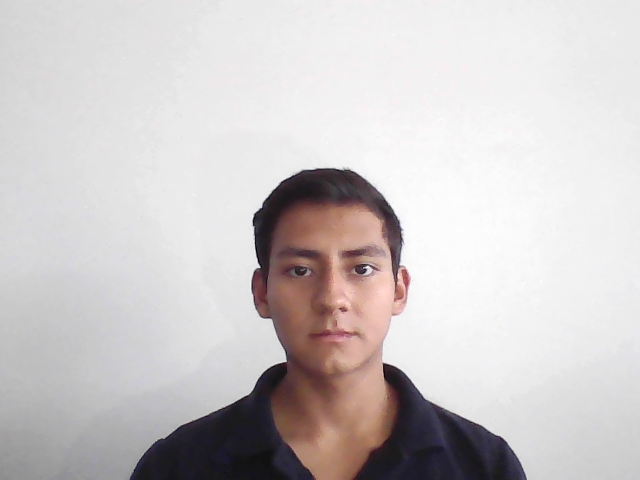
\includegraphics[width=\textwidth]{images/2022630467_new.png}
		\caption{Imagen registrada en el sistema (ej., Imagen de Registro)}
		\label{fig:primera_imagen}
	\end{subfigure}
	\hfill % Para distribuir el espacio horizontalmente
	\begin{subfigure}[b]{0.3\textwidth}
		\centering
		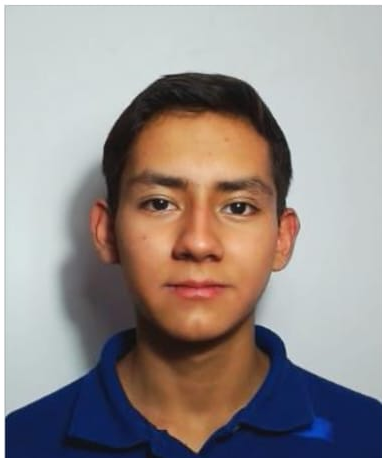
\includegraphics[width=\textwidth]{images/2022630467_old_crop.png} 
		\caption{Imagen de prueba (ej., Imagen de Prueba)}
		\label{fig:segunda_imagen}
	\end{subfigure}
	\caption{Conjunto de imágenes mostrando un ejemplo de imagen de registro y su correspondiente imagen de prueba.}
	\label{fig:conjunto_imagenes}
\end{figure}

%--------------------------------------------------------



